\vfill 
\chapter{Analyse et spécification des besoins}
\label{chap:analyse-specification-besoins}
\mtcaddchapter
\section*{Introduction}
\justifying
L’étape d’analyse et spécification des besoins est une étape indispensable dans la méthode 2TUP pour comprendre les fonctionnalités que le système doit fournir. Ce chapitre sera consacré à détailler cette étape: Nous commencerons par l’identification des acteurs. Puis, nous élaborons le diagramme de contexte de notre système. Ensuite, nous allons faire un recueil sur  les besoins fonctionnels et non fonctionnels de notre projet. Ci-après, nous allons spécifier et analyser les besoins identifiés en se basant sur le modèle de cas d’utilisation et le diagramme de séquence d'analyse du langage  \textbf{U}nified  \textbf{M}odeling  \textbf{L}anguage \textbf{(UML)}. Enfin, un recueil sur les besoins techniques sera présenté tout en citant les frameworks choisis.


\section{Identification des acteurs}
\justifying
Un acteur est une entité externe qui définit le rôle joué par un utilisateur, humain ou non humain, qui interagit avec un système interactif \cite{acteur}.\\
Notre système comporte les acteurs suivants:
\begin{itemize}[itemsep=2pt, parsep=2pt]
    \item \textbf{Etudiant}: L'étudiant, en tant qu'utilisateur inscrit, est au cœur de notre système qui peut interagir avec notre chatbot Mixture of Experts et bénéficier de ses services intelligents. Ainsi, il peut accéder aux salons virtuels (Classrooms) et leurs contenus auxquels il est affilié  c-à-d les ressources pédagogiques de ses enseignants. Ensuite, cet utilisateur peut partager des supports pédagogiques (de ses enseignants ou provenant de sources externes) dans un espace de chat instantané, sollicitant ainsi d'une gamme de services intelligents tels que l'explication, la traduction, la correction d'exercices, la génération de résumés, etc. Ces fonctionnalités sont conçues pour clarifier ses cours, assurant une assistance personnalisée tout au long de son apprentissage.
    \item \textbf{Enseignant}:  L'acteur enseignant est un utilisateur qui admet un compte et joue un rôle actif dans l'expérience d'apprentissage en ligne en facilitant le partage de connaissances et en favorisant un environnement collaboratif au sein de notre plateforme. Ainsi, il bénéficie d'outils conviviaux lui permettant de créer et de gérer des classrooms dédiés à ses cours et y partage ses ressources pédagogiques (cours, fascicule, corrections des fascicules, etc..). Il peut organiser les ressources pédagogiques de manière structurée, favorisant ainsi un accès facile et une interaction fluide avec les étudiants.
    \item \textbf{Modèle MoE (Modèle Mixture of Experts)}:  Le modèle Mixture Of Experts est un composant système qui permet de répondre aux questions et requêtes des étudiants en se basant sur les ressources pédagogiques publiées sur la plateforme ou provenant de sources externes et ainsi de clarifier leurs lacunes. En analysant les matériaux pédagogiques, le modèle fournit des explications détaillées et des exemples pertinents pour clarifier les concepts difficiles offrant un soutien individualisé aux étudiants et améliorant leur compréhension du contenu éducatif.
\end{itemize}

\section{Modèle informationnel de contexte}
\justifying
Le modèle informationnel de contexte donne un aperçu global de notre plateforme en identifiant les acteurs et leurs interactions avec le système. À travers le diagramme de contexte, nous illustrons ces échanges pour une meilleure compréhension. Cette représentation simplifiée du fonctionnement de notre application aide à saisir les flux d'informations et le rôle des différents intervenants.\\
La Figure \ref{fig:diagramme de context} montre le diagramme de contexte et illustre bien le modèle informationnel de l'application.

\begin{figure}[H]
    \centering
    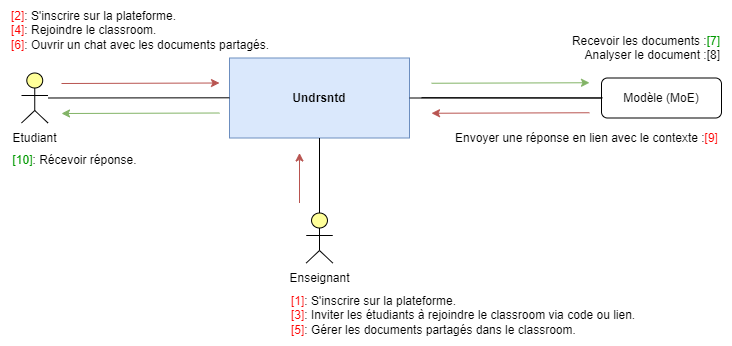
\includegraphics[width=1\textwidth,height=0.35\textheight]{images/chp3/fig1.png}
    \caption{Diagramme de contexte dynamique de notre plateforme}
    \label{fig:diagramme de context}    
\end{figure}
\section{Recueil des besoins}
\justifying
Dans cette section, nous allons présenter les besoins fonctionnels et non fonctionnels de notre plateforme.

\subsection{Capture des besoins fonctionnels}
\justifying
Les besoins fonctionnels définissent les actions que notre système doit accomplir pour répondre aux attentes des utilisateurs. Nous identifions ces besoins en fonction des différents acteurs impliqués. Cette étape nous permet de délimiter le périmètre fonctionnel de notre application et de garantir sa conformité aux exigences des utilisateurs.
\begin{itemize}[itemsep=2pt, parsep=2pt]
    \item \textbf{Besoins fonctionnels de l'étudiant :} 
    \begin{itemize}[itemsep=1pt, parsep=1pt]
        \item \textbf{S'inscrire: }Permettre à l'étudiant de créer un compte sur la plateforme en fournissant des informations nécessaires.
        \item \textbf{S'identifier : }Permettre à l’étudiant de se connecter à son compte pour accéder aux fonctionnalités de la plateforme.
        \item \textbf{Accéder au classroom : } Permettre à l'étudiant de rejoindre et quitter les classrooms, d’ouvrir ou télécharger les documents partagés, de démarrer un chat avec le modèle dans le contexte des documents partagés et d'interagir avec les publications.
        \item \textbf{Démarrer chat : }Permettre à l'étudiant de créer un espace de communication instantanée avec notre chatbot. Dans cette espace, l'étudiant peut non seulement démarrer une nouvelle conversation mais aussi consulter son historique et poursuivre la communication dans une conversation existante. Cette fonctionnalité lui permet d’envoyer une requête en se référant à un document spécifique ou sans faisant référence. Le premier cas est préconditionné par l’importation d’un document dans la conversation courante. 
        \item \textbf{Gérer propre média : }Permettre à l'étudiant de consulter ses documents partagés ainsi que de les supprimer de la base de données.
        \item \textbf{Consulter historique: }Permettre à l’étudiant de consulter l’historique des classrooms, des commentaires ou des postes.
        \item \textbf{Gérer profil : } Permettre à l'étudiant de mettre à jour et de gérer les informations de son profil utilisateur telles que ses informations personnelles et ses préférences ainsi que de supprimer son profil.
    \end{itemize}
    \item \textbf{Besoins fonctionnels de l'enseignant :}
    \begin{itemize}[itemsep=1pt, parsep=1pt]
        \item \textbf{S'inscrire: }Permettre à l'enseignant de créer un compte sur la plateforme en fournissant des informations nécessaires.
        \item \textbf{S'identifier : }Permettre à l'enseignant de se connecter à son compte pour accéder aux fonctionnalités de la plateforme.
        \item \textbf{Gérer classroom : }Permettre à l'enseignant de créer, modifier, archiver, désarchiver et supprimer ses classrooms.
        \item \textbf{Accéder au classroom : } Permettre à l'enseignant de gérer des publications en créant, modifiant et supprimant des publications, d'ouvrir ou télécharger des documents partagés, d'inviter des étudiants au classroom et d'interagir sur les publications.
        \item \textbf{Consulter historique: } Permettre à l’enseignant de consulter l’historique des classrooms, des commentaires ou des postes.
        \item \textbf{Gérer profil :  } Permettre à l'enseignant de mettre à jour et de gérer les informations de son profil utilisateur telles que ses informations personnelles et ses préférences ainsi que de supprimer son profil.
    \end{itemize}
    \item \textbf{Besoins fonctionnels du modèle MoE :}
    \begin{itemize}[itemsep=1pt, parsep=1pt]
        \item \textbf{Répondre à une requête : } Permettre au modèle (MoE) de générer des réponses pertinentes en se référant à un document importé par l'étudiant ou à des ressources externes. Le modèle (MoE) est capable de traiter divers types de documents tels que des textes, des articles, des livres et même des codes sources. En fonction de cette analyse approfondie, il peut non seulement répondre aux questions de l'étudiant, mais, aussi, accomplir une multitude de tâches supplémentaires. Ainsi, il peut générer des résumés condensés des documents pour faciliter la compréhension, expliquer des concepts difficiles et donner des exemples concrets, corriger les exercices en fournissant des explications détaillées et bien plus encore…
    \end{itemize}

\end{itemize}

\subsection{Capture des besoins non fonctionnels}
Les besoins non fonctionnels sont des critères de qualité qui décrivent les attentes non liées, directement, aux  comportements fonctionnels.\\
Les besoins non fonctionnels de notre système sont:
\begin{itemize}[itemsep=1pt, parsep=1pt]
    \item \textbf{La sécurité : }L'application doit garantir à l'utilisateur connecté l'intégrité et la confidentialité de ses données.
    \item \textbf{La convivialité : }La conception de l’interface utilisateur doit être simple et intuitive permettant aux utilisateurs de naviguer facilement dans le système et d’accomplir leurs tâches de manière efficace et agréable.
    \item \textbf{La performance : }Le système doit être en mesure de fournir des performances rapides et efficaces.
    \item \textbf{Fiabilité : }L’application doit fonctionner de façon cohérente pour les utilisateurs.
    \item \textbf{Rapidité : }Le système doit traiter les requêtes en temps réel et fournir des réponses instantanées aux étudiants pour répondre à leurs besoins. 
\end{itemize}

\section{Spécification des besoins }
Pour une meilleure documentation de notre plateforme, nous allons formaliser, dans cette section, les fonctionnalités offertes par notre application en utilisant le diagramme de cas d'utilisation de l’UML.

\subsection{Diagramme de cas d’utilisation global}
Le diagramme de cas d'utilisation est le mécanisme le plus populaire pour la spécification des exigences. Il illustre les interactions entre les acteurs et le système. En outre, il donne une vue d'ensemble des fonctionnalités que le système doit offrir pour répondre aux besoins des utilisateurs.\\
La Figure \ref{fig:diagramme de cas d’utilisation global} illustre le diagramme de cas d’utilisation global de notre plateforme.

\begin{figure}[H]
    \centering
    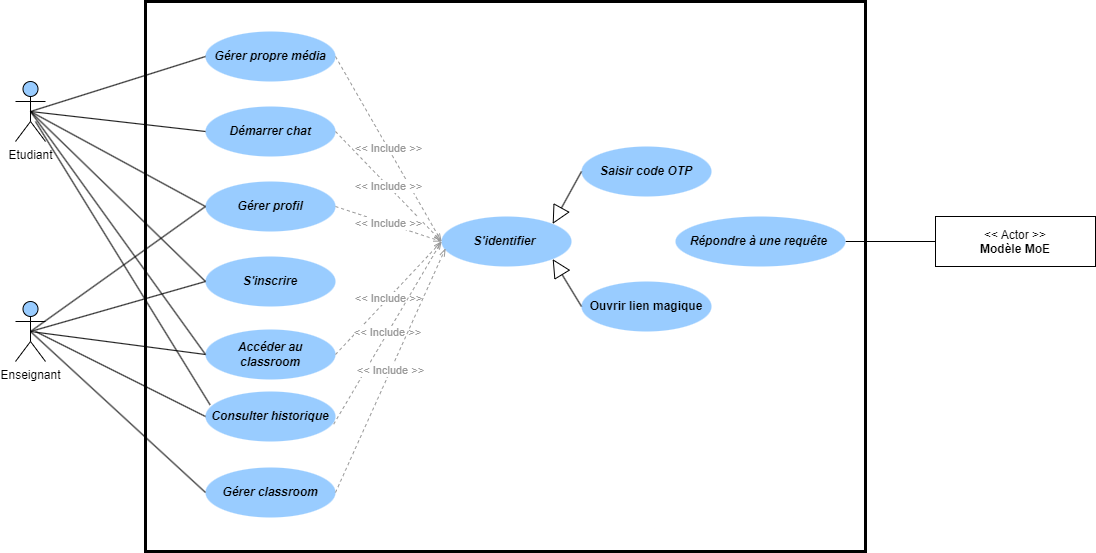
\includegraphics[width=1.1\textwidth,height=0.75\textheight]{images/chp3/fig2.png}
    \caption{Diagramme de cas d’utilisation global}
    \label{fig:diagramme de cas d’utilisation global}    
\end{figure}

\subsection{Diagrammes de cas d’utilisation détaillés}
Dans cette partie, nous allons raffiner les cas d'utilisation présentés dans la Figure \ref{fig:diagramme de cas d’utilisation global}. Le raffinement sera représenté par un diagramme de cas d'utilisation détaillé de chaque  acteur.

\subsubsection{Diagramme de cas d’utilisation détaillé de l’acteur << Etudiant >>}
La Figure \ref{fig:diagramme de cas d’utilisation détaillé de l’acteur << Etudiant >>} illustre le diagramme de cas d’utilisation détaillé de l’acteur étudiant après avoir s’identifier.
\begin{figure}[H]
    \centering
    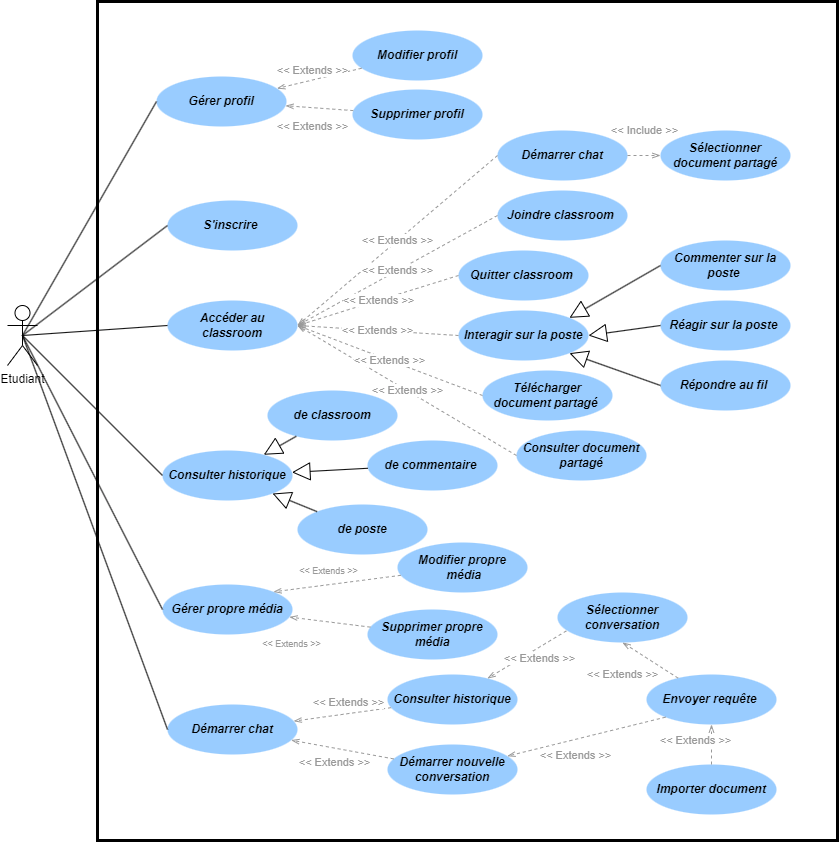
\includegraphics[width=1.1\textwidth,height=0.85\textheight]{images/chp3/fig3.png}
    \caption{Diagramme de cas d’utilisation détaillé de l’acteur << Etudiant >>}
    \label{fig:diagramme de cas d’utilisation détaillé de l’acteur << Etudiant >>}    
\end{figure}

\subsubsection{Diagramme de cas d’utilisation détaillé de l’acteur << Enseignant >>}
La Figure \ref{fig:diagramme de cas d’utilisation détaillé de l’acteur << Enseignant >>} illustre le diagramme de cas d’utilisation détaillé de l’acteur enseignant après avoir s’identifier.
\begin{figure}[H]
    \centering
    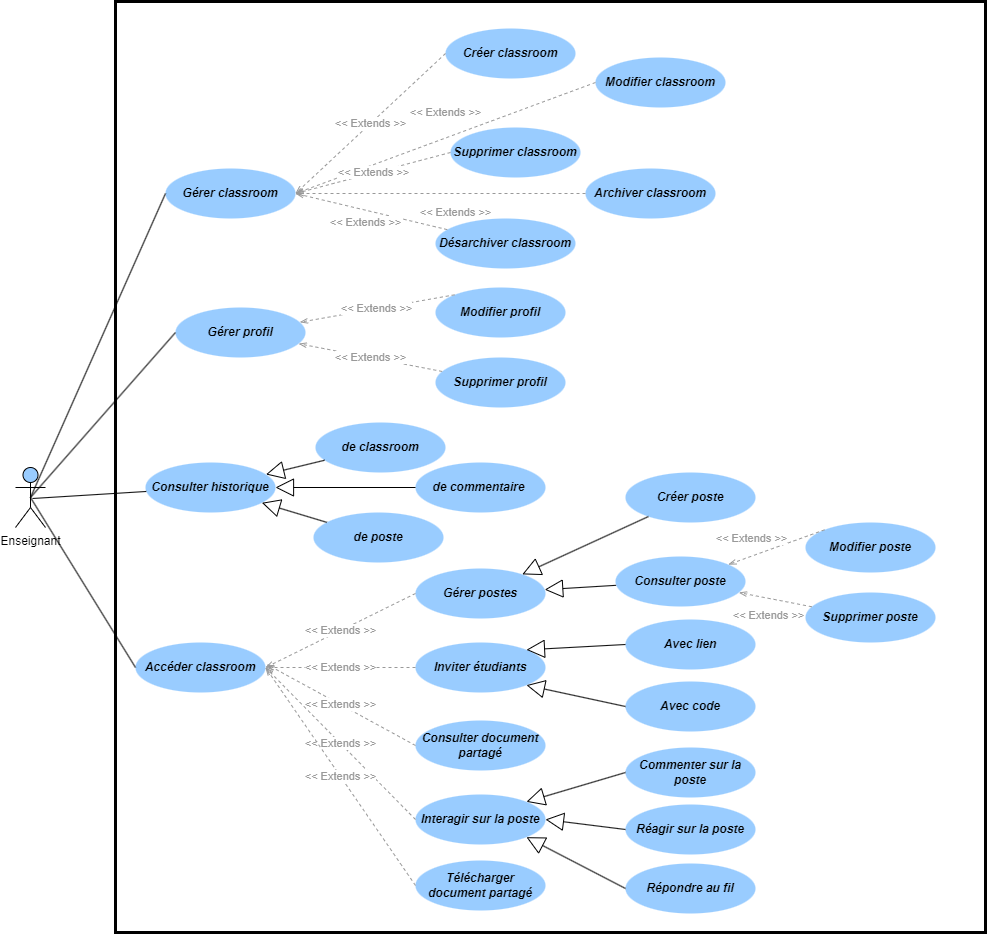
\includegraphics[width=1.1\textwidth,height=0.85\textheight]{images/chp3/fig4.png}
    \caption{Diagramme de cas d’utilisation détaillé de l’acteur << Enseignant >>}
    \label{fig:diagramme de cas d’utilisation détaillé de l’acteur << Enseignant >>}    
\end{figure}


\subsubsection{ Diagramme de cas d’utilisation détaillé de l’acteur << Modèle MoE >>}
La Figure \ref{fig: Diagramme de cas d’utilisation détaillé de l’acteur <<Modèle MoE>>>} illustre le diagramme de cas d’utilisation détaillé de l’acteur modèle MoE.

\begin{figure}[H]
    \centering
    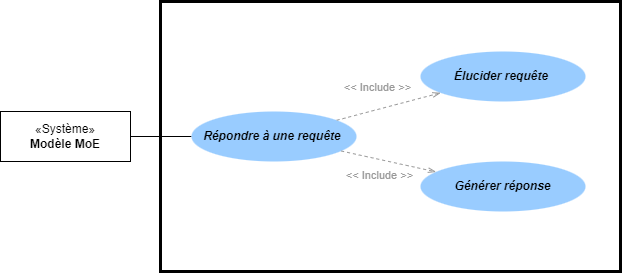
\includegraphics[width=\textwidth,height=0.3\textheight]{images/chp3/fig5.png}
    \caption{Diagramme de cas d’utilisation détaillé de l’acteur <<Modèle MoE>>}
    \label{fig: Diagramme de cas d’utilisation détaillé de l’acteur <<Modèle MoE>>>}    
\end{figure}

\subsection{Analyse des besoins}
L'analyse des besoins est une étape importante permettant de représenter le comportement du système au fil du temps. Dans le contexte de la modélisation orienté objet, l’analyse des besoins peut se faire par les descriptions textuelles et les diagrammes de séquence d'analyse. Une description textuelle est description des scénarios nominaux, d'extension et d'exception d’un cas d'utilisation. Un diagramme de séquence d'analyse, dite aussi acteur-système, est une représentation graphique utilisée pour montrer l’interaction entre les acteurs et le système où le système est représenté sous d'une boîte noire. Dans cette section, nous présenterons les descriptions textuelles et les diagrammes de séquence d'analyse relatifs aux principaux cas d’utilisation de notre plateforme.

\subsubsection{Cas d’utilisation << S’identifier >> }
\begin{itemize}[itemsep=1pt, parsep=1pt]
    \item \textbf{Description textuelle}\\
    Le tableau 3.1 montre la description textuelle du cas d’utilisation \textbf{<< S’identifier >>}.
\newpage
    \begin{longtable}{|>{\RaggedRight\arraybackslash}p{4cm}|>{\RaggedRight\arraybackslash}p{12cm}|}
        \caption{Description textuelle du cas d’utilisation « S’identifier »} \\
        \hline
        \textbf{Titre de cas d’utilisation} & \textbf{S’identifier} \\
        \hline
        \textbf{Acteurs principaux} & Utilisateur (Enseignant, Étudiant) \\
        \hline
        \textbf{Description} & Grâce à ce cas d’utilisation, un utilisateur peut s’identifier et accéder à notre plateforme. \\
        \hline
        \textbf{Précondition} & L’utilisateur doit avoir un email universitaire. \\
        \hline
        \textbf{Postcondition} & L’utilisateur doit avoir un compte sur la plateforme. \\
        \hline
        \textbf{Scénarios nominaux} & 
        \begin{itemize}[label=]
            \item \textbf{Scénario nominal 1: Se connecter}
            \begin{enumerate}
                \item L’utilisateur accède à la page de connexion.
                \item L’utilisateur saisit son email universitaire.
                \item L’utilisateur essaie de se connecter en appuyant sur le bouton \textbf{\textit{‘Se connecter’}}.
                \item Si le champ mail est vide, l’\textbf{\textit{Exception 1}} se déclenche.
                \item Le système envoie un email \textbf{O}ne \textbf{T}ime \textbf{P}assword \textbf{(OTP)} à l’email universitaire propre de l’utilisateur avec un code OTP et un lien magique.
                \item L’utilisateur choisit une méthode de connexion: 
                \begin{itemize}[label=--]
                    \item \textbf{Via un lien magique :} L’utilisateur clique sur le lien magique dans l’email.
                    \item \textbf{Via la saisie du code OTP :} L’utilisateur entre le code OTP dans le champ de la saisie du code OTP. Si le code est erroné, l'\textbf{\textit{Exception 2}} se déclenche.
                \end{itemize}
                \item Le système affiche la page principale de la plateforme.
            \end{enumerate}
            \item \textbf{Scénario nominal 2: Se déconnecter}
            \begin{enumerate}
                \item L’utilisateur clique sur son avatar.
                \item L’utilisateur se déconnecte en cliquant sur le bouton \textbf{\textit{‘Se déconnecter’}}.
                \item Le système affiche la page de connexion.
            \end{enumerate}
        \end{itemize} \\
        \hline
        \textbf{Scénarios alternatifs} & 
        \begin{enumerate}
            \item L’utilisateur accède à la page de connexion.
            \item L’utilisateur essaie de se connecter en appuyant sur le bouton \textbf{\textit{‘Github’}}. 
            \item Le système affiche la page principale de la plateforme. \newline \textbf{Notez bien} que l'utilisateur doit utiliser son email universitaire comme email principal et publique sur son compte GitHub.
        \end{enumerate} \\
        \hline
        \textbf{Exceptions} & 
        \begin{itemize}[label=--]
            \item \textbf{\textit{Exception 1}} : Si l’utilisateur ne remplit pas le champ email, un message d’erreur \textit{<< Le champ email est requis >>} est affiché.
            \item \textbf{\textit{Exception 2}} : Si l’utilisateur saisit un code erroné, un message d’erreur \textit{<< Le code est invalide >>} est affiché.
        \end{itemize} \\
        \hline
    \end{longtable}
    \label{tab:Description textuelle du cas d’utilisation « s’identifiere »}

    \newpage
    \item \textbf{Diagramme de séquence acteur-système}\\
     Pour ce cas d'utilisation, l'utilisateur peut être soit un étudiant, soit un enseignant lors de l'identification.\\
     La Figure \ref{fig:diagramme de séquence << S’identifier >>} illustre le diagramme de séquence \textbf{<< S’identifier >>}.
     \begin{figure}[H]
        \centering
        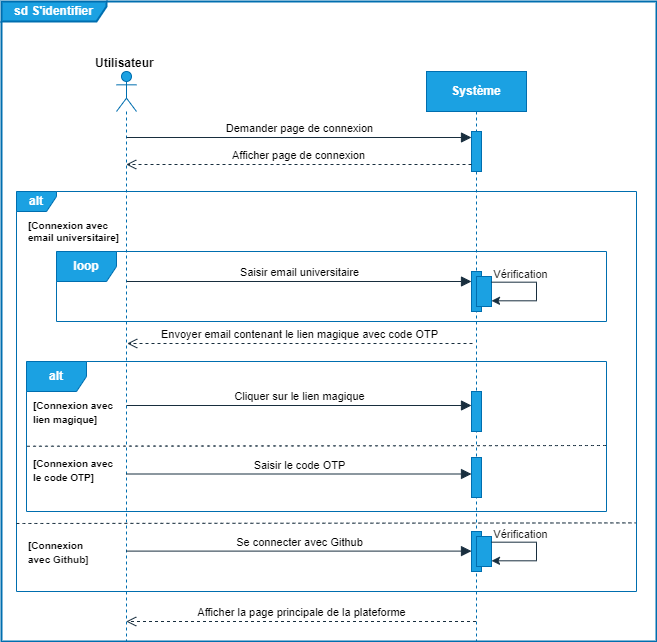
\includegraphics[width=1.1\textwidth,height=0.82\textheight]{images/chp3/fig6.png}
        \caption{Diagramme de séquence << S’identifier >>}        
        \label{fig:diagramme de séquence << S’identifier >>}    
    \end{figure}

\end{itemize}

\subsubsection{Cas d’utilisation << Gérer classroom >>}
\begin{itemize}[itemsep=1pt, parsep=1pt]
    \item \textbf{Description textuelle}\\
    Le tableau 3.2 montre la description textuelle du cas d’utilisation \textbf{<< Gérer classroom >>}.
    \begin{longtable}{|>{\RaggedRight\arraybackslash}p{4cm}|>{\RaggedRight\arraybackslash}p{12cm}|}
        \caption{ Description textuelle du cas d’utilisation << Gérer classroom >> } \\
        \hline
        \textbf{Titre de cas d’utilisation} & \textbf{Gérer classroom} \\
        \hline
        \textbf{Acteurs principaux} & Enseignant \\
        \hline
        \textbf{Description} & Grâce à ce cas d’utilisation, un enseignant peut créer, modifier, supprimer, archiver et désarchiver un classroom. \\
        \hline
        \textbf{Précondition} & Enseignant identifié. \\
        \hline
        \textbf{Postcondition} & La liste des classrooms est mise à jour avec les modifications apportées (création, modification, suppression, archivage, désarchivage du classroom). \\
        \hline
        \textbf{Scénarios nominaux} & 
        \begin{itemize}[label=]
            \item \textbf{Scénario nominal: Créer classroom}
            \begin{enumerate}
                \item L’enseignant demande la page de classrooms.
                \item Le système affiche la liste des classrooms pour l’enseignant. 
                \item L’enseignant clique sur le bouton \textbf{\textit{‘Créer classroom’}}.
                \item Le système affiche le formulaire d’ajout d’un classroom. 
                \item L’enseignant remplit le formulaire de la création du nouveau classroom.
                \item 
                \begin{enumerate}
                    \item S’il existe un champ vide, l’\textbf{\textit{Exception 1}} s’affiche. 
                    \item Si un champ ne vérifie pas sa contrainte, l’\textbf{\textit{Exception 2}} s’affiche.
                \end{enumerate}
                \item Le système ajoute le classroom dans la base de données.
            \end{enumerate}
        \end{itemize} \\
        \hline
        \textbf{Scénarios alternatifs} & 
        \begin{itemize}[label=]
            \item \textbf{Scénario alternatif 1: Modifier classroom}
            \begin{enumerate}
                \item L’enseignant demande la page de classrooms.
                \item Le système affiche la liste des classrooms pour l’enseignant. 
                \item L’enseignant clique sur le bouton de la modification du classroom spécifié.
                \item Le système affiche le formulaire de modification du classroom.  
                \item L’enseignant modifie les informations du classroom à modifier. 
                \item 
                \begin{enumerate}
                    \item S’il existe un champ vide, l’\textbf{\textit{Exception 1}} s’affiche. 
                    \item Si un champ ne vérifie pas sa contrainte, l’\textbf{\textit{Exception 2}} s’affiche.
                \end{enumerate}
                \item Le Système modifie les informations du classroom dans la base de données.
            \end{enumerate}
            \item \textbf{Scénario alternatif 2: Supprimer classroom}
            \begin{enumerate}
                \item L’enseignant demande la page de classrooms.
                \item Le système affiche la liste des classrooms pour l’enseignant. 
                \item L’enseignant clique sur le bouton de suppression de classroom spécifié.
                \item Le système affiche une fenêtre superposée pour confirmer la suppression. 
                \item L’enseignant clique sur le bouton \textbf{\textit{‘Confirmer’}}.
                \item Le système retire le classroom de la base de données.
            \end{enumerate}
        \end{itemize} \\
        \hline
        \textbf{Scénarios alternatifs} & 
        \begin{itemize}[label=]
            \item \textbf{Scénario alternatif 3: Archiver classroom }
            \begin{enumerate}
                \item L’enseignant demande la page de classrooms.
                \item Le système affiche la liste des classrooms pour l’enseignant. 
                \item L’enseignant clique sur le bouton d’archivage de classroom spécifié.
                \item Le système affiche une fenêtre superposée pour confirmer l’archivage. 
                \item L’enseignant clique sur le bouton \textbf{\textit{‘Confirmer’}}.
                \item Le système archive le classroom.
            \end{enumerate}
            \item \textbf{Scénario alternatif 4: Désarchiver classroom }
            \begin{enumerate}
                \item L’enseignant demande la page de classrooms.
                \item Le système affiche la liste des classrooms pour l’enseignant. 
                \item L’enseignant clique sur le bouton de désarchivage de classroom spécifié.
                \item Le système affiche une fenêtre superposée pour confirmer le désarchivage.
                \item L’enseignant clique sur le bouton \textbf{\textit{‘Confirmer’}}.
                \item Le système désarchive le classroom.
            \end{enumerate}
        \end{itemize} \\
        \hline
        \textbf{Exceptions} & 
        \begin{itemize}[label=--]
            \item \textbf{\textit{Exception 1}} : Si l’enseignant ne remplit pas un ou plusieurs champs du formulaire, un message d’erreur spécifique est affiché pour chaque champ vide. 
            \item \textbf{\textit{Exception 2}} : Si l’enseignant remplit un ou plusieurs champs du formulaire mais que les contraintes ne sont pas vérifiées, un message d’erreur spécifique est affiché pour chaque champ invalide.
        \end{itemize} \\
        \hline
    \end{longtable}
    \newpage
    \item \textbf{Diagramme de séquence acteur-système}\\
    La Figure 3.7 illustre le diagramme de séquence \textbf{<< Créer classroom >>}.
     \begin{figure}[H]
        \centering
        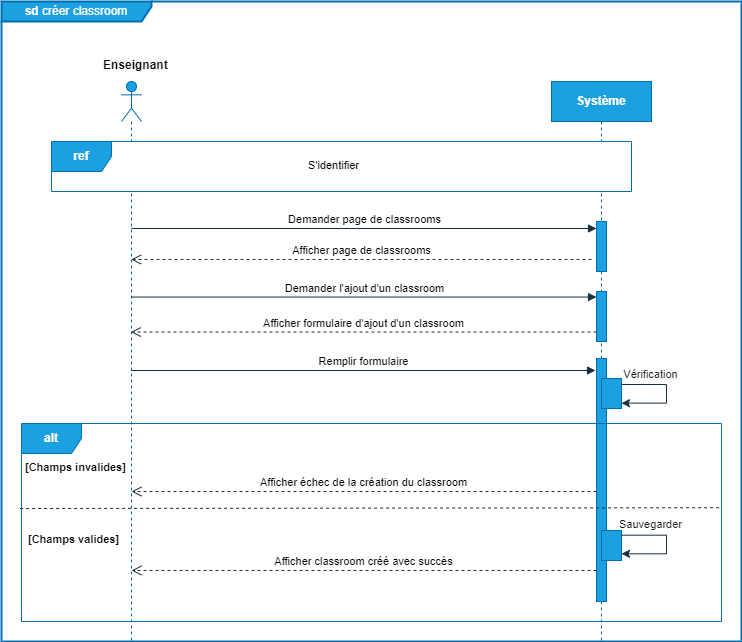
\includegraphics[width=1.1\textwidth,height=0.85\textheight]{images/chp3/fig7.png}
        \caption{Diagramme de séquence << Créer classroom >>}        
        \label{fig:Diagramme de séquence << Créer classroom >>}    
    \end{figure}

\end{itemize}

\subsubsection{ Cas d’utilisation << Démarrer chat >>}
\begin{itemize}[itemsep=1pt, parsep=1pt]
    \item \textbf{Description textuelle}\\
    Le tableau 3.3 montre la description textuelle du cas d’utilisation \textbf{<< Démarrer chat >>}.
    \begin{longtable}{|>{\RaggedRight\arraybackslash}p{4cm}|>{\RaggedRight\arraybackslash}p{12cm}|}
        \caption{Description textuelle du cas d’utilisation << Démarrer chat >>} \\
        \hline
        \textbf{Titre de cas d’utilisation} & \textbf{Démarrer chat} \\
        \hline
        \textbf{Acteurs principaux} & Etudiant \\
        \hline
        \textbf{Description} & Grâce à ce cas d’utilisation, un étudiant peut créer une conversation avec le modèle MoE dans notre plateforme. Il peut envoyer des questions, des requêtes (demande d’explication, traduction, synthèse, etc.) sur un document partagé avec le système. \\
        \hline
        \textbf{Précondition} & Étudiant identifié. \\
        \hline
        \textbf{Postcondition} & Conversation créée. \\
        \hline
        \textbf{Scénarios nominaux} &    
        \begin{enumerate}
            \item L’étudiant demande la page de chat avec le modèle MoE.
            \item Le système affiche au étudiant la page de chat.
            \item L’étudiant clique sur le bouton \textbf{\textit{‘Conversations’}}.
            \item Le système affiche liste des conversations précédentes. 
            \item L’étudiant choisit la manière de communication:
            \begin{itemize}[label=--]
                \item Conversation en tenant les conversations précédentes:
                \begin{itemize}[label=5.1.]
                    \item L’étudiant sélectionne une conversation (conversation x)
                \end{itemize}
                \item L’étudiant veut démarrer une nouvelle conversation: 
                \begin{itemize}[label=5.1.]
                    \item L’étudiant remplit le formulaire d’une nouvelle conversation.
                \end{itemize}
            \end{itemize}
            \item L’étudiant communique avec le modèle.
            \item Le système élucide les demandes de l’étudiant:
            \begin{itemize}[label=--]
                \item Réponse en se référant aux ressources externes: Le modèle génère les réponses de l'étudiant en utilisant les informations provenant de ressources externes mentionnées.
                \item Réponse en se référant aux ressources internes: Le modèle génère les réponses de l'étudiant en se basant sur les informations et le contexte mentionnés dans le document partagé, tout en permettant une explication plus approfondie en se référant à des ressources externes.
            \end{itemize}
            \item Le système envoie les réponses.
        \end{enumerate}\\
        \hline
        \textbf{Exceptions} & 
        \begin{itemize}[label=--]
            \item \textbf{\textit{Exception 1}} : Si l’étudiant importe un document de format invalide, le système affiche un message d’erreur \textit{<< Fichier invalide, veuillez vérifier le format de fichier >>}.
            \item \textbf{\textit{Exception 2}} : Si la taille de document dépasse 25 Méga octets, le système affiche un message d’erreur \textit{<< Veuillez réduire la taille du document pour continuer >>}.
        \end{itemize} \\
        \hline
    \end{longtable}
    
    \item \textbf{Diagramme de séquence acteur-système}\\
    La Figure 3.8 illustre le diagramme de séquence \textbf{<< Démarrer chat >>}.
     \begin{figure}[H]
        \centering
        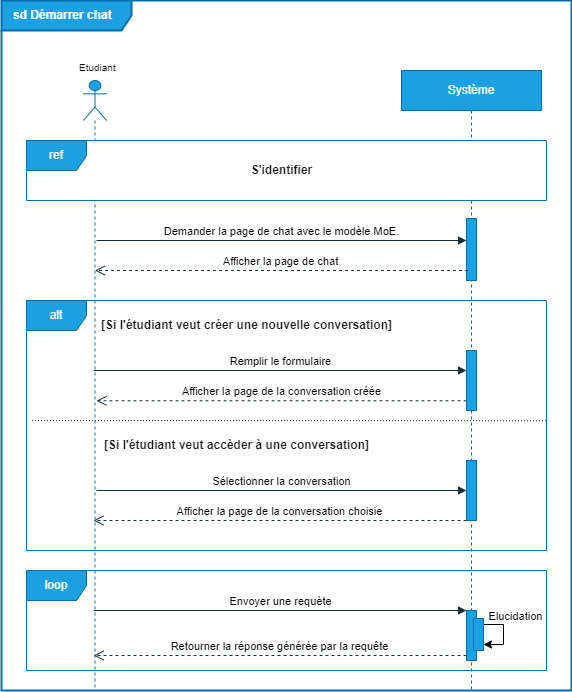
\includegraphics[width=1.1\textwidth,height=0.85\textheight]{images/chp3/fig8.png}     
           \caption{Diagramme de séquence << Démarrer chat >>}        
        \label{fig:Diagramme de séquence << Démarrer chat >>}    
    \end{figure}
    
\end{itemize}

\section{Capture des besoins techniques}
Dans cette section, nous allons présenter les logiciels et outils utilisés pour développer et mettre en œuvre notre plateforme. Nous allons mettre en valeur le Framework utilisé pour le développement frontend et backend ainsi que la base de donnée choisie pour notre projet.

\subsection{Framework frontend}
\noindent Pour la partie frontend, nous allons utiliser le framework Next.js.
\vspace{0.5em}
\begin{wrapfigure}{l}{0.08\linewidth}
    \vspace{-15pt}
    
\includegraphics[width=0.1\textwidth]{images/chp5/nextjs.png}
\end{wrapfigure}
\textbf{Next.js} est un framework gratuit et open source s'appuyant sur la bibliothèque javascript React. Next.js se distingue par sa capacité à offrir une expérience utilisateur performante et réactive. Grâce à sa structure basée sur React, Next.js permet de construire des interfaces utilisateur dynamiques et interactives avec une facilité. Son approche basée sur le rendu côté serveur garantit des performances optimales. Il offre aussi ses fonctionnalités avancées telles que le pré rendu des pages et le routage dynamique facilitant la navigation fluide et la gestion efficace des données.\\
La Figure 3.9 présente les statistiques de la satisfaction des utilisateurs à l’usage des frameworks et bibliothèques dans le domaine du développement web.
    \begin{figure}[H]
        \centering
        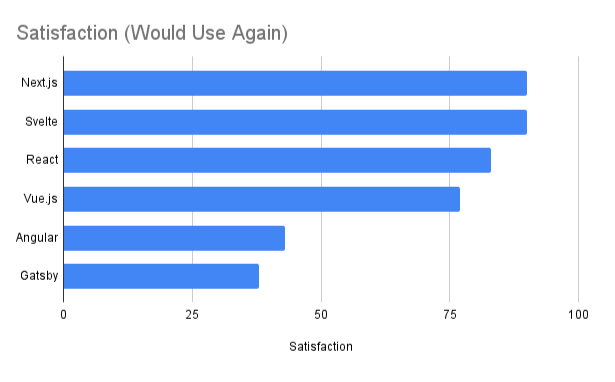
\includegraphics[width=1\textwidth,height=0.4\textheight]{images/chp3/fig9.png}
        \caption{Les statistiques de la satisfaction des utilisateurs à l’usage des frameworks et bibliothèques dans le domaine du développement web \cite{StatsFramework}}        
        \label{fig:Les statistiques de la satisfaction des utilisateurs à l’usage des frameworks et bibliothèques dans le domaine du développement web}    
    \end{figure}

\subsection{Framework backend}
\noindent Next.js est souvent associé au développement frontend en raison de sa capacité à créer des interfaces utilisateur réactives et performantes. Il offre également des fonctionnalités robustes pour la partie backend. Grâce à sa compatibilité avec Node.js, Next.js permet de développer facilement des applications web full-stack en combinant efficacement le frontend et le backend. L'utilisation de Next.js pour la partie backend offre plusieurs avantages comme la possibilité de créer des API RESTful, la gestion des bases de données et la mise en œuvre de la logique métier côté serveur. Avec son architecture flexible et sa facilité d'utilisation, Next.js permet aux développeurs de créer des applications web complètes et cohérentes en offrant ainsi une expérience utilisateur fluide et satisfaisante pour la partie frontend et aussi la partie backend.

\subsection{Base de données}
\noindent Pour notre système de gestion de base de données, nous avons opté pour une approche SQL en utilisant PostgreSQL. Cette décision découle des nombreux avantages offerts par les bases de données SQL telles que la robustesse des transactions et la gestion efficace des données structurées.
\vspace{0.5em}
\begin{wrapfigure}{l}{0.1\linewidth}
    \vspace{-15pt}
    
\includegraphics[width=0.1\textwidth]{images/chp5/postgresql.png}
\end{wrapfigure}
\textbf{PostgreSQL }est un système de gestion de base de données relationnelle open source qui offre une performance robuste, une fiabilité élevée et une extensibilité exceptionnelle. Connu pour sa conformité aux normes SQL, PostgreSQL prend en charge une large gamme de fonctionnalités avancées telles que les jointures complexes, les transactions \textbf{ACID} (\textbf{A}tomicité, \textbf{C}ohérence, \textbf{I}solation, \textbf{D}urabilité) et la réplication asynchrone. Il est préféré pour être un choix pour les développeurs et les entreprises qui cherchent une solution de base de données puissante et fiable pour leurs applications.\\
La Figure 3.10 présente les statistiques des options de base de données les plus populaires.
    \begin{figure}[H]
        \centering
        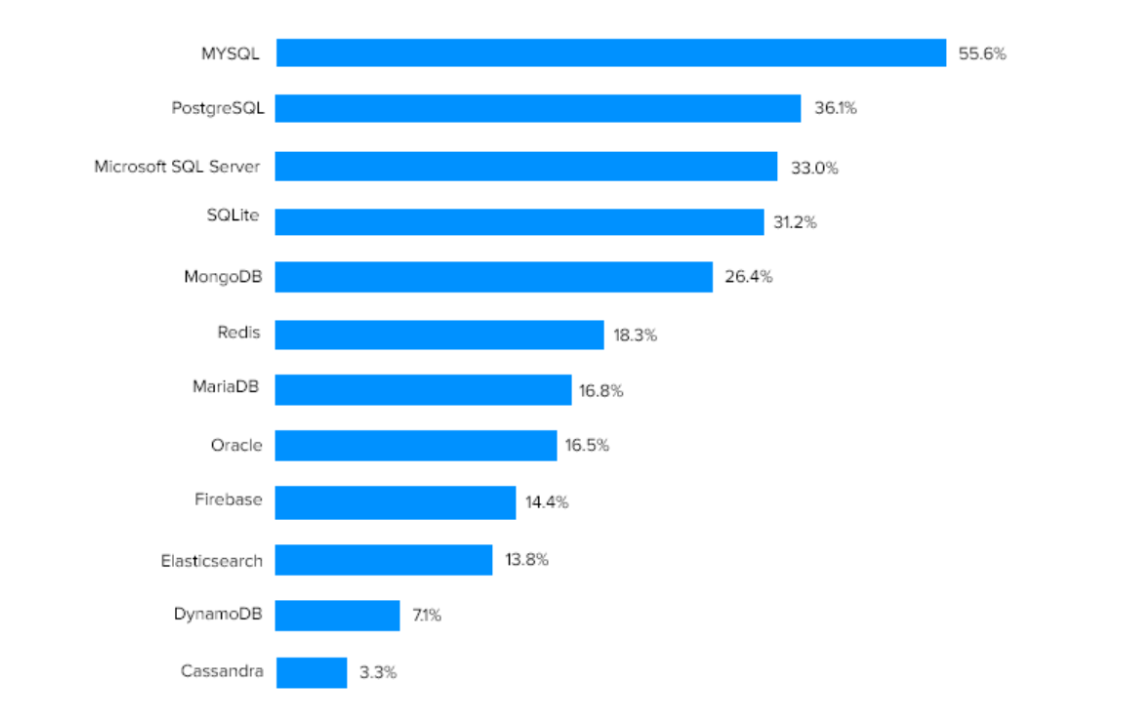
\includegraphics[width=1.2\textwidth,height=0.4\textheight]{images/chp3/fig10.png}
        \caption{Les statistiques des options de base de données les plus populaires \cite{StatsBdd}}      
        \label{fig:Les statistiques des options de base de données les plus populaires}    
    \end{figure}
    
\section*{Conclusion}
Dans ce chapitre, nous avons mis en œuvre les branches fonctionnelle et technique de la méthode 2TUP en utilisant le modèle de cas d'utilisation (diagramme et description textuelle) et le diagramme de séquence d'analyse. Dans le chapitre suivant, nous présenterons la conception préliminaire et détaillée de notre application en appliquant la branche de la réalisation de la méthode 2TUP.